\let\negmedspace\undefined
\let\negthickspace\undefined
\documentclass[journal]{IEEEtran}
\usepackage[a4paper, margin=10mm, onecolumn]{geometry}
%\usepackage{lmodern} % Ensure lmodern is loaded for pdflatex
\usepackage{tfrupee} % Include tfrupee package

\setlength{\headheight}{1cm} % Set the height of the header box
\setlength{\headsep}{0mm}  % Set the distance between the header box and the top of the text

\usepackage{gvv-book}
\usepackage{gvv}
\usepackage{cite}
\usepackage{amsmath,amssymb,amsfonts,amsthm}
\usepackage{algorithmic}
\usepackage{graphicx}
\usepackage{float}
\usepackage{textcomp}
\usepackage{xcolor}
\usepackage{txfonts}
\usepackage{listings}
\usepackage{enumitem}
\usepackage{mathtools}
\usepackage{gensymb}
\usepackage{comment}
\usepackage[breaklinks=true]{hyperref}
\usepackage{tkz-euclide} 
\usepackage{listings}
% \usepackage{gvv}                                        
\def\inputGnumericTable{}                                 
\usepackage[latin1]{inputenc}                                
\usepackage{color}                                            
\usepackage{array}                                            
\usepackage{longtable}                                       
\usepackage{calc}                                             
\usepackage{multirow}                                         
\usepackage{hhline}                                           
\usepackage{ifthen}                                           
\usepackage{lscape}
\usepackage{tikz}
\usetikzlibrary{patterns}

\begin{document}

\bibliographystyle{IEEEtran}
\vspace{3cm}

\title{1.1.6.13}
\author{ee25btech11063-vejith}

\maketitle
% \maketitle
% \newpage
% \bigskip
{\let\newpage\relax\maketitle}
\renewcommand{\thefigure}{\theenumi}
\renewcommand{\thetable}{\theenumi}
\setlength{\intextsep}{10pt} % Space between text and floats
\textbf{Question}:\\
The points $\brak{0,5}$,$\brak{0,-9}$ and $\brak{3,6}$ are  not collinear.
\\
\textbf{Solution: }\\
\begin{table}[h!]    
  \centering
  \begin{center}
\begin{tabular}{ll}
    \textbf{Group I} & \textbf{Group II} \\
    P. Ferrite & 1. Hexagonal Close Packed (HCP) \\
    Q. Austenite & 2. Body Centered Cubic (BCC) \\
    R. Martensite & 3. Body Centered Tetragonal (BCT) \\
    & 4. Face Centered Cubic (FCC)
\end{tabular}
\end{center}
  \caption{Variables Used}
  \label{}
\end{table}\\
\begin{align}
\text{3 points are collinear if the rank of collinearity matrix is 1.Rank of matrix is 1 means no.of rows with non zero entries is 1.}    
\end{align}

\begin{align}
\text{The collinearity matrix is given by}\\
\myvec{
   \vec{B}-\vec{A} & \vec{C}-\vec{A}
 }^T = \myvec{
   0 & -14 
   \\
   3 & 1
   }\\
\end{align}
\begin{align}
    \myvec{
   0 & -14 
   \\
   3 & 1
   }
  &\xrightarrow{R_1 \leftrightarrow R_2}
   \myvec{
   3 & 1
   \\
   0 & -14
   }\\
 \end{align}
 The above matrix now is in row echelon form.Rank of a matix in echelon form is number of non zero rows.so,The rank of the above collinearity matrix is 2\\
 $\implies$ given 3 points A,B,C are not collinear.
 \begin{figure}[h!]
   \centering
   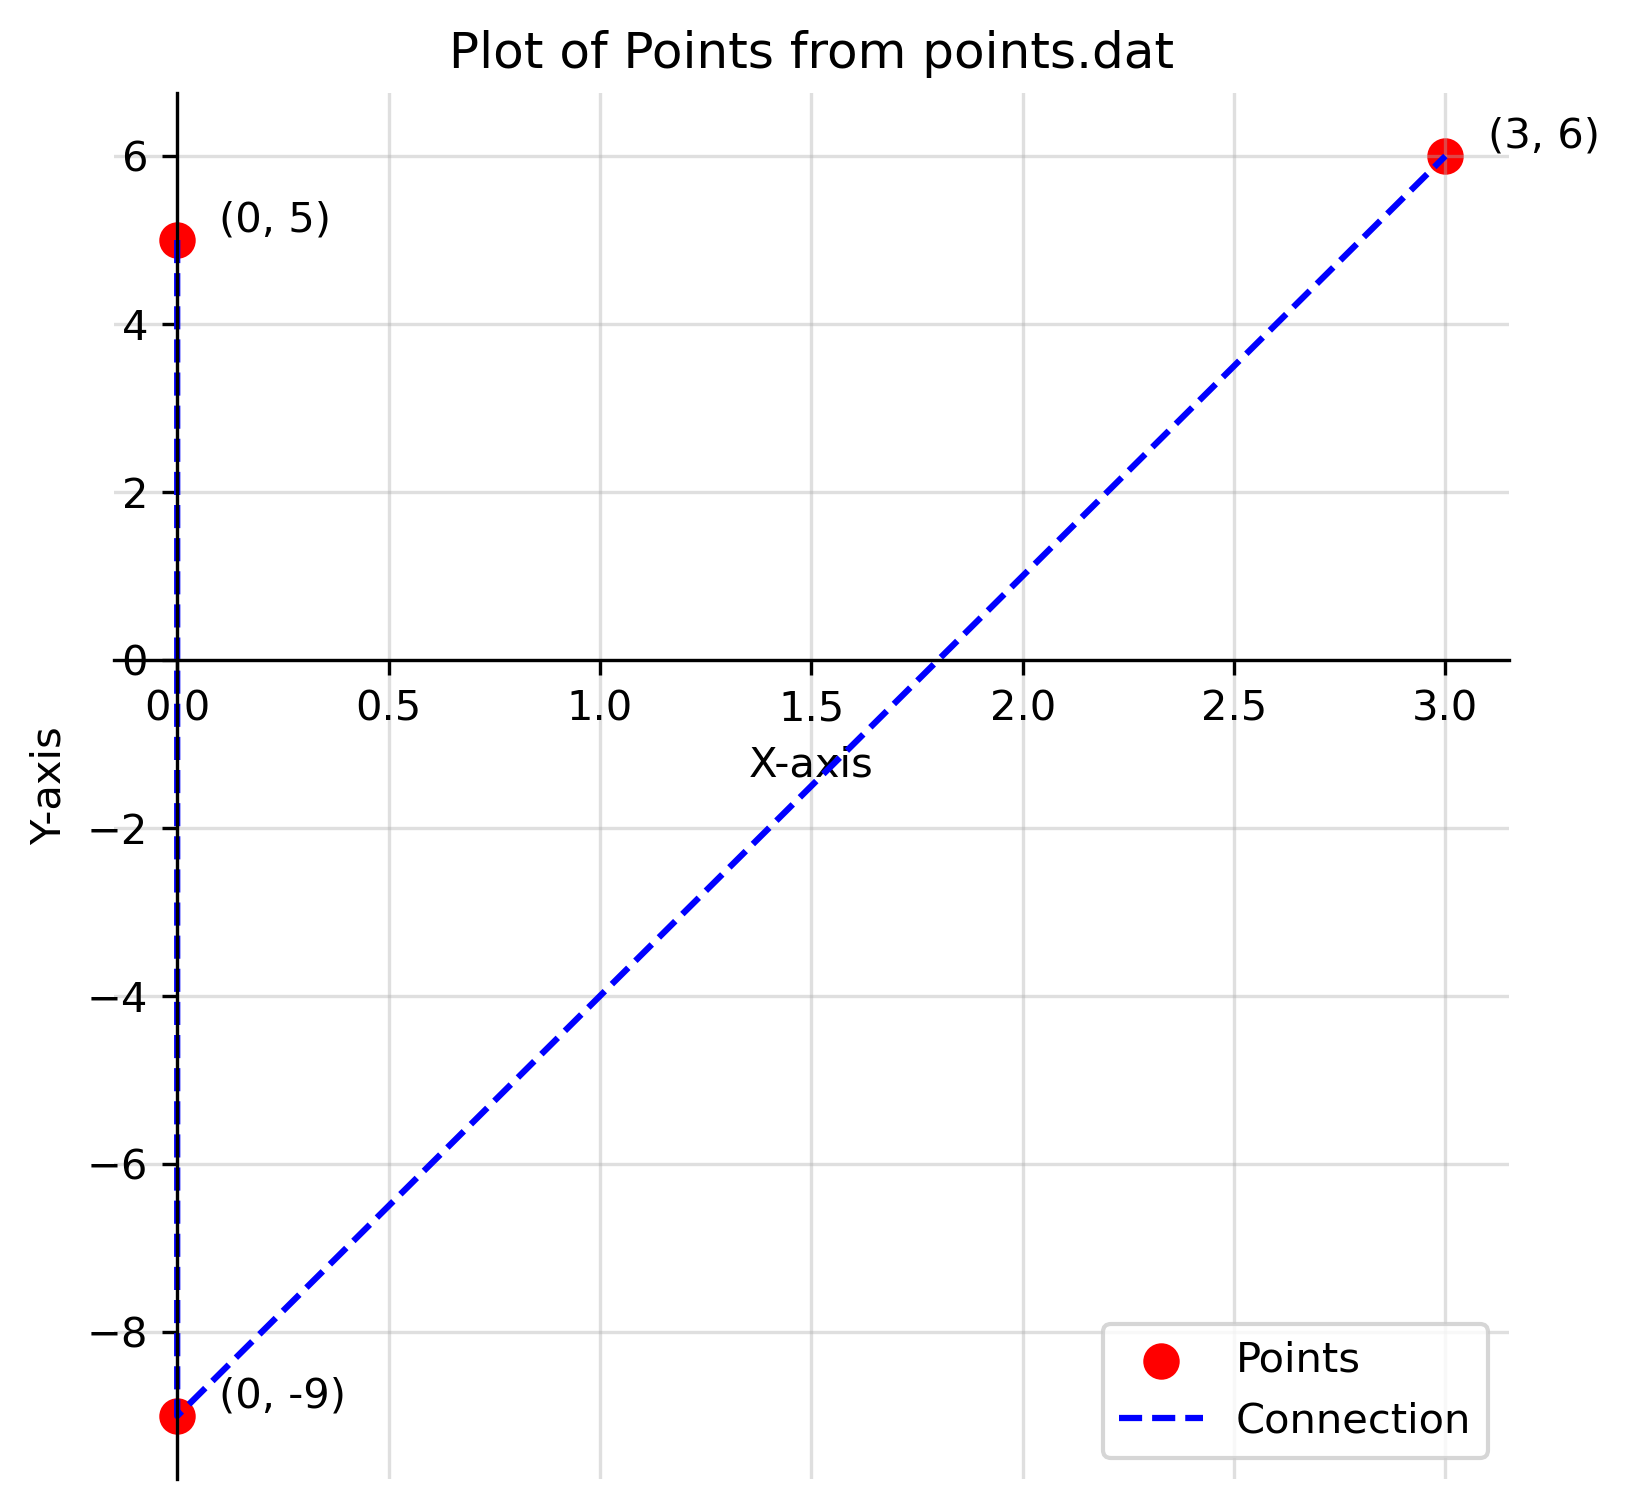
\includegraphics[width=0.5\linewidth]{figs/01.png}
   \caption{Triangle formed by points A,B,C}
   \label{}
\end{figure}
\end{document}
